% !TeX encoding = UTF-8
% !TeX root = master.tex
% !TeX spellcheck = en_US

\documentclass{styles/llncs}

\usepackage[utf8]{inputenc}
\usepackage[T1]{fontenc}
\usepackage[english]{babel}
\selectlanguage{english}
\usepackage{graphicx}
\usepackage{grffile}
\graphicspath{{figures/}}
\usepackage{float}
\usepackage{booktabs}
\usepackage{tabu}
\usepackage{rotating}
\usepackage{array}
\usepackage{multirow}
\usepackage{url}
\usepackage{footnote}
\usepackage{footmisc}
\usepackage[hidelinks]{hyperref} %[draft,hidelinks]
\usepackage[all]{hypcap}
\usepackage[capitalise,noabbrev,nameinlink]{cleveref}
\crefname{section}{Sect.}{Sect.}
\Crefname{section}{Section}{Sections}
\crefname{figure}{Fig.}{Fig.}
\Crefname{figure}{Figure}{Figures}
\usepackage[nonumberlist,acronym,nomain]{glossaries}
\usepackage[gen]{eurosym}
\usepackage{etoolbox}
\glsdisablehyper
\makeglossaries

\makeatletter
\g@addto@macro{\UrlBreaks}{\UrlOrds}
\makeatother

\newtoggle{ebib}
\togglefalse{ebib} %toogle to true for extended bibliography

\newacronym{ann}{ANN}{Artificial Neural Networks}
\newacronym{atm}{ATM}{Automated Teller Machine}
\newacronym{brief}{BRIEF}{Binary Robust Independent Elementary Features}
\newacronym{brisk}{BRISK}{Binary Robust Invariant Scalable Keypoints}
\newacronym{clahe}{CLAHE}{Contrast Limited Adaptive Histogram Equalization}
\newacronym{fast}{FAST}{Features from Accelerated Segment Test}
\newacronym{freak}{FREAK}{Fast Retina Keypoint}
\newacronym{flann}{FLANN}{Fast Library for Approximate Nearest Neighbors}
\newacronym{hmm}{HMM}{Hidden Markov Models}
\newacronym{gftt}{GFTT}{Good Features to Track}
\newacronym{mser}{MSER}{Maximally Stable Extremal Regions}
\newacronym{opencv}{OpenCV}{Open Source Computer Vision}
\newacronym{orb}{ORB}{Oriented FAST and Rotated BRIEF}
\newacronym{ransac}{RANSAC}{Random Sample Consensus}
\newacronym{sift}{SIFT}{Scale Invariant Feature Transform}
\newacronym{surf}{SURF}{Speeded Up Robust Features}
\newacronym{svm}{SVM}{Support Vector Machines}



\begin{document}



%---------------------------------------------------------------------------------------------------
% Top matter
%---------------------------------------------------------------------------------------------------

\title{Recognition of Banknotes in Multiple Perspectives Using Selective Feature Matching and Shape Analysis}

\author{%
	\IEEEauthorblockN{Carlos M. Costa}
	\IEEEauthorblockA{INESC TEC\\
		and Faculty of Engineering,\\
		University of Porto\\
		Email: carlos.m.costa@inesctec.pt
	}
	\and
	\IEEEauthorblockN{Germano Veiga}
	\IEEEauthorblockA{INESC TEC\\
		Email: germano.veiga@inesctec.pt
	}
	\and
	\IEEEauthorblockN{Armando Sousa}
	\IEEEauthorblockA{INESC TEC\\
		and Faculty of Engineering,\\
		University of Porto\\
		Email: asousa@fe.up.pt
	}
}

\IEEEtitleabstractindextext{%
	\begin{abstract}

Reliable banknote recognition is critical for detecting counterfeit banknotes in ATMs and help visual impaired people. To solve this problem, it was implemented a computer vision system that can recognize multiple banknotes in different perspective views and scales, even when they are within cluttered environments in which the lighting conditions may vary considerably. The system is also able to recognize banknotes that are partially visible, folded, wrinkled or even worn by usage. To accomplish this task, the system relies on computer vision algorithms, such as image preprocessing, feature detection, description and matching. To improve the confidence in the recognition results, the feature matching results are used to compute the contour of the banknotes using an homography, that later on is validated using shape analysis algorithms. The system successfully recognized all Euro banknotes in 80 test images, even when there were several overlapping banknotes in the same test image.

\keywords{banknote recognition $\cdot$ feature matching $\cdot$ computer vision $\cdot$ shape analysis}

\end{abstract}

	\begin{IEEEkeywords}
		banknote recognition, feature matching, computer vision, shape analysis
	\end{IEEEkeywords}
}

\maketitle
\IEEEdisplaynontitleabstractindextext



%---------------------------------------------------------------------------------------------------
% Sections
%---------------------------------------------------------------------------------------------------

\section{Introduction}\label{sec:introduction}

Banknotes play a critical role in our trading society, and although digital currency is becoming more popular, physical banknotes still account for a large amount of the local transactions. As such, systems that are able to recognize banknotes can be applied to aid in the manipulation of this type of currency.

These kind of systems are critical to visually impaired people, since they allow them to be more independent while avoiding the help of untrusted people. Also, they can increase the security and reliability of ATMs \cite{Sako2007}, by making sure the maintenance operations are performed correctly and the valid banknotes are not replaced with counterfeits. Other less critical applications are related with automatic sorting and counting of banknotes to speedup transactions and money transfers.

For these types of systems to be effective and useful, they must be able to recognize the banknotes in several perspective views, scale dimensions, and should also tolerate cluttered environments with different lighting conditions. Besides these critical requirements, in order to be properly used to help visually impaired people, they should also be able to recognize folded, wrinkled and worn banknotes.

For the implementation of the robust banknote recognition system, the input images are preprocessed to remove environment noise and improve contrast and brightness. Then important keypoints and their associated descriptors are computed, to later be used to find the best matching in a database of valid banknotes. The correct matching of keypoint descriptors is critical to ensure the proper recognition of the banknotes. As such, methods to filter the inliers from the matches are employed. There are several techniques to perform such filtering, such as the ratio test (presented in section 7.1 of \cite{Lowe2004}) and the homography outlier removal (chapter 3 of \cite{Baggio2012}). Although these techniques can yield very good results, a postprocessing analysis is applied to make sure the results obtained are really banknotes. This is related to the fact that the matching of several parts of wrinkle banknotes may result in the recognition of multiple instances of the same banknote. In addition, images similar to banknotes or from other countries banknotes may yield incorrect partial matches. As such, this postprocessing phase is critical to ensure the correct recognition of the banknotes. It starts by computing the banknote contour using the retrieved homography, and then removes any result that has a convex contour, or has its area, circularity and aspect ratio outside the acceptable ranges for banknotes. To detect multiple banknotes in the same image, the inliers of the last recognized banknote are removed and the process presented earlier is repeated until there are no more valid matches.

In the following section it will be presented an overview of the several approaches that can be used to perform banknote recognition. In \cref{sec:implementation} a detailed description of the implementation will be provided. In \cref{sec:results} the representative results of the recognition system will be provided and in \cref{sec:results-analysis} it will be discussed the robustness of the system. Finally, the conclusions will be given in \cref{sec:conclusions}.

\section{Related Work}\label{sec:related-work}

There are several approaches that can be used to successfully recognize banknotes [4], and they range from simple but less robust techniques to more advanced and accurate systems.

The simplest technique is to use template matching to try to find the banknotes in the image by simple bitmap comparison. But this has the problem that both the reference banknotes and targets in the image must have the same size and perspective view. To mitigate this restriction, the comparison could be done in several scales and orientations, but it wouldn't be very efficient. The dynamic template matching proposed in [5] could be used instead, but it still isn't the best way to handle the recognition.

Other way to tackle this problem would be to perform color and shape segmentation of specific parts of the banknotes, like the method proposed in [6]. But this can complicate the implementation since it would have to be tuned to each specific banknote, and it would require a lot of effort to successfully recognize all banknotes from both sides.

A more broad implementation could use the size, color and texture of each banknote to perform the recognition [7], but like the previous case, it would require fine tuning to recognize each banknote, and would have to take in consideration the accuracy of the distance measurements, because several banknotes may have similar sizes.

A more robust implementation could use Principal Component Analysis or even adapt the eigenfaces algorithm to try to recognize the banknotes [8], but this can have some problems when the perspective of the reference banknotes is very different from the ones in the image.

For detection of counterfeit banknotes, ultra violet or infra-red light could be used to highlight specific parts of the banknotes that are hard to duplicate and easier to recognize [9]. Other similar technique takes advantage of the fact that specific parts of the banknotes are highlighted when they are illuminated with LEDs with different colors and intensities [10]. And another approach takes in consideration the electromagnetic fields present in sections of the banknotes to perform the recognition [11]. But all these techniques require special hardware that is too expensive. Moreover, they are not meant to be used by visually impaired people.

One of the most common techniques applied to banknote recognition uses machine learning algorithms, such as Support Vector Machines [12]–[14], Artificial Neural Networks [15]–[17], and Hidden Markov Models [18], [19]. These techniques usually apply some sort of clustering of features before training the classifier, such as the Bag of Keypoints model [20], or try to extract relevant features from the reference images. After the training, the classifiers can be used to recognize the banknotes. Although this is a good approach to general recognition, it may not be very precise in calculating the exact location and contour of the banknotes.

After the state of art review, it was considered that the technique that was likely to have the best results, and could be efficiently implemented, had to rely in algorithms that detected important features in the reference banknotes. Moreover, these features should be able to be correctly matched in the test images even if the banknotes were in different perspectives and in different lighting conditions. As such, an approach based in detection of edges [21], corners [22], blobs [23] and even ridges, could yield the identification of keypoints that could be successfully matched in the conditions presented earlier. For this matching to succeed, a scale and rotation invariant descriptor should be computed for each keypoint, using for example SIFT [2] or SURF [24] algorithms. After this matching, an outlier removal step could be applied to improve the accuracy of the detection, and the final recognition could be analyzed to make sure it was really recognized a banknote. This kind of approach has proved that it can achieved very good results, as shown in [25]–[27].

\section{Implementation}\label{sec:implementation}

In the following sections the main steps of the implemented banknote recognition system will be presented. The C++ source code along with the complete results are available at \footnote{\url{https://github.com/carlosmccosta/Currency-Recognition}}. To speed up development, the \gls{opencv} library was used.


\subsection{Preprocessing}

To improve the detection of good features and ensure that the system has robust recognition even when the images have considerable noise, a preprocessing step is applied.

In a first phase, most of noise is removed using a bilateral filter\iftoggle{ebib}{ \cite{Tomasi1998}}. This filter was chosen because it preserves the edges of the image blobs, which are very valuable structures in the detection of feature points.

After the noise is reduced, a \gls{clahe} \iftoggle{ebib}{\cite{Heckbert1994}} is applied to increase the contrast. This can improve the recognition of the system when the images are taken in low light environments. This technique has better results over the simple histogram equalization because it can be applied to images that have areas with high and low contrast, and also limits the spread of the noise.

Finally, the brightness is adjusted to correct images that are too dark or too bright.

\Cref{fig:preprocessing} shows the impact of the preprocessing stage in an image which had noise caused by the wrinkled plastic.

\begin{figure}[H]
	\centering
	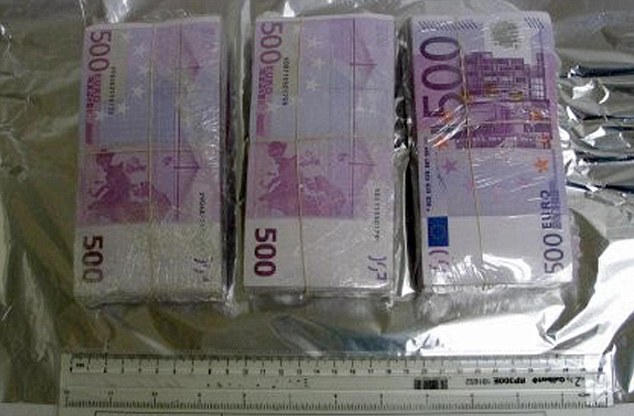
\includegraphics[width=.498\textwidth]{preprocessing/before-500-500-500}\hfill
	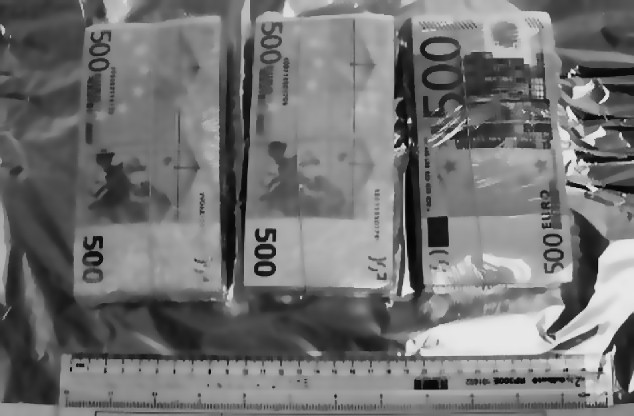
\includegraphics[width=.498\textwidth]{preprocessing/after-500-500-500}
	\caption{Impact of preprocessing stage (original image on the left, preprocessed image on the right)}
	\label{fig:preprocessing}
\end{figure}


\subsection{Reference image database setup}

In order for the system to be able to recognize the target banknotes, a database of valid instances must be computed.

This database contains the descriptors associated with the keypoints for each banknote (from both sides). These descriptors are calculated in the same way as presented in section \cref{sec:feature-detection} and \cref{sec:keypoint-descriptor-extraction} and the images are also preprocessed.

To improve the detection of the relevant parts of the banknotes and to avoid the usage of sections that are similar across several banknotes, the keypoint detection algorithm is only applied inside the masks associated with each banknote. Only relevant parts such as the banknote number and unique textures or patterns are included in the banknotes masks (only the white areas shown in \cref{fig:banknote-feature-detection-mask-500-front} will be used to compute the keypoints of a 500\,\euro{} banknote).


\begin{figure}[H]
	\centering
	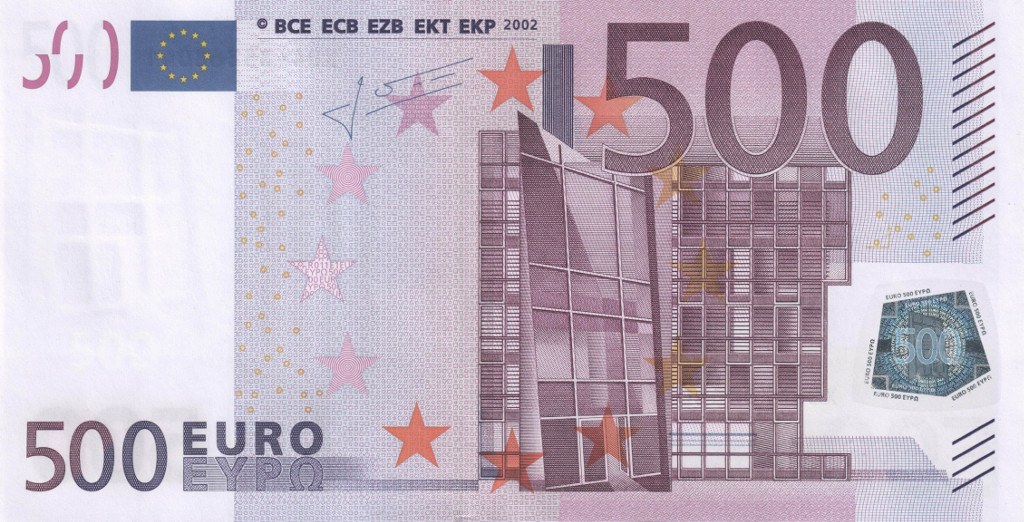
\includegraphics[width=.2499\textwidth]{notes-masks/500eu-front}\hfill
	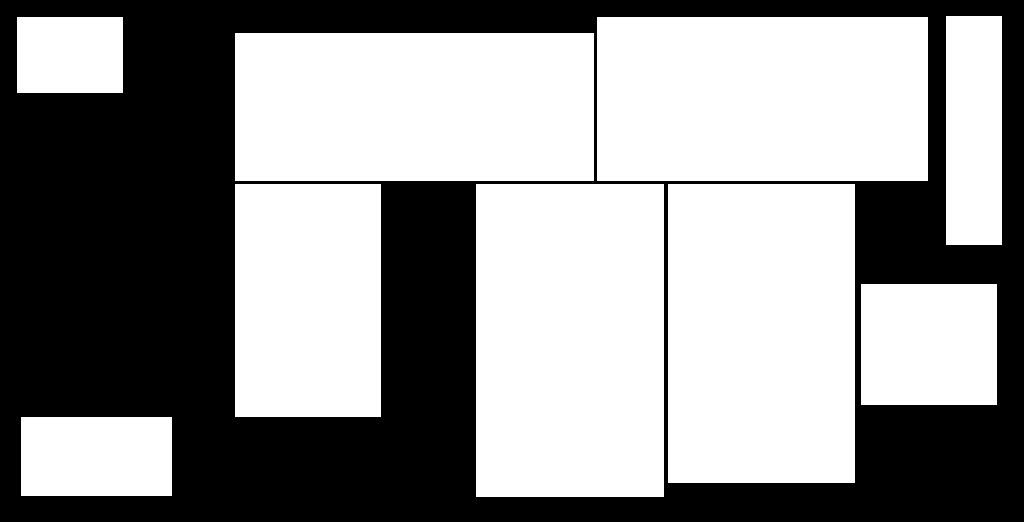
\includegraphics[width=.2499\textwidth]{notes-masks/500eu-front-mask}\hfill
	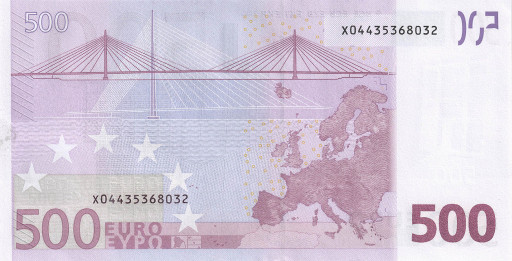
\includegraphics[width=.2499\textwidth]{notes-masks/500eu-back}\hfill
	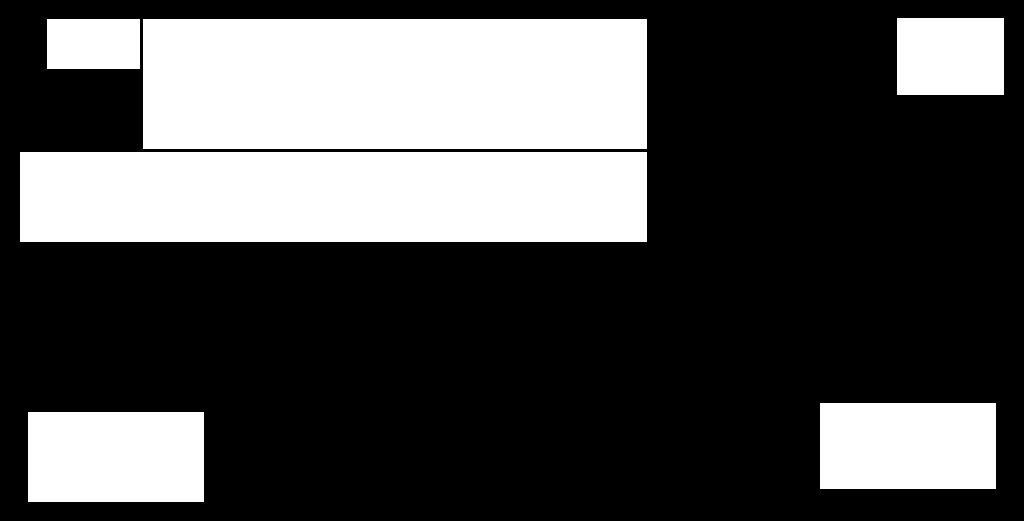
\includegraphics[width=.2499\textwidth]{notes-masks/500eu-back-mask}
	\caption{Front and back of a 500\,\euro{} banknote with associated feature detection masks}
	\label{fig:banknote-feature-detection-mask-500-front}
\end{figure}


\subsection{Recognition}

The recognition is the most critical phase in the system, in which the provided image is analyzed to extract the banknotes monetary value and their contour.

The current implementation supports recognition of multiple banknotes in the same image, even if they are partially occluded.

The system was implemented to recognize any type of banknotes. The Euro currency was selected for the computation of the results, but any other currency can be used. To setup the system for other currencies it is only necessary to replace the database images and masks with the intended currency images.

To improve the robustness of the system, 3 levels of detail for each banknote are provided (with images having pixel width of 256, 512 and 1024 respectively).

For an ideal banknote recognition result, the image resolution of both the reference and the target images should be the same. But converting a high resolution banknote database to the image banknotes resolution has a considerable processing overhead, and as such, to allow the system to be more efficient and able to run in real time, a compromise between precision and computation time was achieved by precomputing the reference images in 3 different scales. At run time, the appropriate level of detail is selected according to the resolution of the target image.

The reason for several levels of details is related to the fact that the geometry of the banknotes changes drastically from a low resolution to a high resolution banknote image. As a result, the computed keypoints and their associated descriptors will be considerably different and the recognition of the banknotes will likely fail. This can be clearly seen in \cref{fig:banknote-500-front-resolution-difference}. This approach mitigates this problem by selecting the most similar database image resolution in relation to the banknotes in the image being analyzed.

\begin{figure}[H]
	\centering
	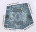
\includegraphics[width=.2499\textwidth]{image-resolution/500eu-front-very-low}\hfill
	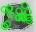
\includegraphics[width=.2499\textwidth]{image-resolution/500eu_front_currencyDB_veryLowResolution_SIFT-Detector}\hfill
	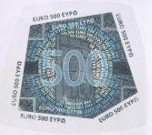
\includegraphics[width=.2499\textwidth]{image-resolution/500eu-front-medium}\hfill
	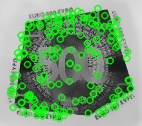
\includegraphics[width=.2499\textwidth]{image-resolution/500eu_front_currencyDB_mediumResolution_SIFT-Detector}
	\caption{Impact of image resolution when computing SIFT keypoints from a very low resolution image (left) to a high resolution image (right) of the hologram of a 500\,\euro{} banknote}
	\label{fig:banknote-500-front-resolution-difference}
\end{figure}


\subsubsection{Feature detection}\label{sec:feature-detection}
Feature detection is the initial recognition step in which interesting keypoints for matching are identified in the image.

These keypoints are normally selected by analyzing the edges, corners, blobs or even ridges. Also, the keypoints provide a condensed representation of the image, which significantly speeds up matching (compared to bitmap or blob matching).

To allow fine tuning of the system, the implementation supports the usage of several feature detection algorithms. Namely, \gls{sift} \cite{Lowe2004}, \gls{surf} \cite{Bay2006}, \gls{gftt} \cite{Shi1994}, \gls{fast} \cite{Rosten2006}, \gls{orb} \cite{Rublee2011}, \gls{brisk} \cite{Leutenegger2011}, STAR \cite{Agrawal2008} and \gls{mser} \cite{Matas2004}.


\subsubsection{Keypoint descriptor extraction}\label{sec:keypoint-descriptor-extraction}

The feature description step associates to each keypoint a description of its surroundings, in order to allow the matching of keypoints. This normally involves the computation of n-jets or local histograms and the final result is a vector in an n-dimensional space characterizing each keypoint.

In order to detect instances with different perspective views, these descriptors must be scale and rotation invariant. Also, they should tolerate different lightning conditions.

There are several algorithms that can accomplish this task, and as such, they were included in the implementation and can be selected to fine tuning the system. It was included the \gls{sift} \cite{Lowe2004}, \gls{surf} \cite{Bay2006}, \gls{freak} \cite{Alahi2012}, \gls{brief} \cite{Calonder2010}, \gls{orb} \cite{Rublee2011} and \gls{brisk} \cite{Leutenegger2011} feature descriptors.


\subsubsection{Descriptors matching and inliers filtering}\label{sec:descriptors-matching-and-inliers-filtering}

In order to detect multiple banknotes in the same image, a correct matching between the image descriptors and the reference banknotes descriptors must be establish. Moreover, these matches should be verified to see if they really belong to a banknote.

The initial matching can be performed using either a brute force or a heuristic approach. In the brute force approach, each descriptor in the image is compared with all descriptors in the reference image to find the best correspondence. In the heuristic approach using the \gls{flann} \cite{Muja2009}, several optimizations are employed to speed up the computations. These optimizations can be related to the appropriate selection of which keypoints to match and to the use of efficient data structures to speed up the search (such as k-d trees).

After the initial matching, an inliers filtering phase is applied. It starts by applying a ratio test (presented in section 7.1 of \cite{Lowe2004}) and then refines the results with the computation of a homography. In the ratio test, each image keypoint descriptor is associated with the two best reference image descriptors. This allows to decide if the matching is correct or not, by computing the ratio between the distances of these references keypoints. The rationale behind it, is that if the ratio is close to 1, then there are two points with equivalent match probability, and as such, is very likely that this is an incorrect match, and should be discarded.

The refinement of the inliers is performed with the computation of a homography that allows the mapping of the positions in the reference image to the positions in the target image, in which the banknotes to be recognize reside. This is achieved by using the \gls{ransac} \iftoggle{ebib}{\cite{Fischler1981}} method to find the homography that best fits the detected keypoints. Since this is a \gls{ransac} method, it iteratively tries to find better results by randomly selecting the supporting keypoints until there is a high confidence in the results or the maximum number of iterations is reached. The rationale behind using such method is that the geometry of the banknotes is planar, and if it is assumed that in most cases the banknotes that are going to be recognize have also planar geometry, then a homography can be used to analyze if a match is correct or not. This classification is performed by applying the homography to the reference keypoints and see if the result position in the target image is close to the position of the matched keypoint. If it is, then the match can be considered correct.

Having the inliers, two approaches can be used to decide if a valid banknote was found or not. One technique relies in the computation of the global inliers ratio in relation to the number of keypoints, and considers that there was a correct match if this ratio is above a given threshold. This is the most appropriate method for most of the banknote recognition cases. Another method that may yield better results when the banknotes are partially occluded, is to consider a correct match when one of the components of the masks (shown in Fig. 1) have the local inliers ratio above a given threshold. The idea behind this approach is to consider each patch of the image represented in the mask as a unique identifier of the banknote. As such, if this local patch is correctly detected, then there is a high confidence that the recognition of that banknote was successful.


\subsubsection{Shape analysis}\label{sec:shape-analysis}

When a banknote matching is considered valid, it undergoes a postprocessing step in which its contour shape is analyzed.

This step is crucial to avoid the multiple detection of the same banknote when it is wrinkled or folded. Also, it removes any recognition that have a contour shape that can't be associated with a banknote.

The initial filtering is performed by removing any result which have a contour with a very low area in relation to the whole image.

In a second step, any result without a convex contour is also removed. This is applied because a banknote has a convex quadrilateral shape. It will never have a concave shape, even when it is folded. The reason for this is that the contour is not computed from the banknote borders. Instead a homography is used to map the 4 corners of the reference image to the positions in the image in which the banknotes reside.

A final step removes any result that has a contour with a circularity or aspect ratio outside the acceptable bounds. These bounds are retrieved from a database of valid shapes (shown in \cref{fig:currency-db-shapes}).

\begin{figure}
	\centering
	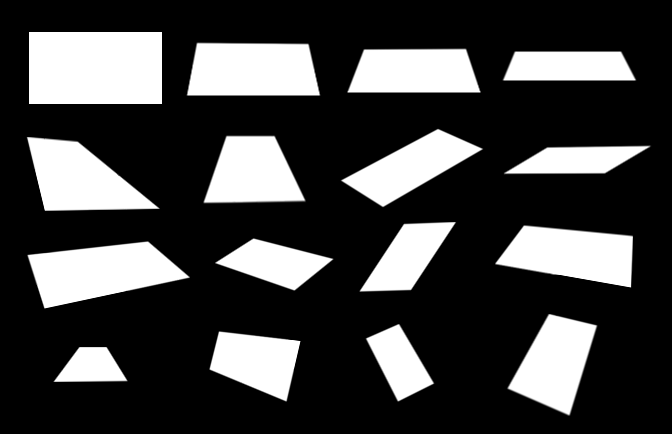
\includegraphics[width=0.87\textwidth]{notes-masks/currency-db-shapes}
	\caption{Database of valid instances of banknote shapes}
	\label{fig:currency-db-shapes}
\end{figure}


\subsubsection{Detection of multiple banknotes}

In order to recognize several banknotes in the same image, the steps presented in \cref{sec:descriptors-matching-and-inliers-filtering,sec:shape-analysis} are performed to every banknote reference image, and the best match is chosen. After the retrieval of the best match, its inliers are removed from the keypoint set, and these two steps (shown in \cref{sec:descriptors-matching-and-inliers-filtering,sec:shape-analysis}) are repeated again for every reference image, in order to find another banknote. This is done until no valid match is found.

Only the inliers must be removed from the keypoint set in order to be able to successful recognize partially occluded banknotes. A less robust method (not used), that will likely fail, removes the keypoints that are inside the banknote contour. Although it might require less computations to perform, it will fail to detect banknotes that are on top of each other, because part of their keypoints will be removed when one of the banknotes is detected.

\section{Results}\label{sec:results}

The system was tested with 80 test images (overview of banknotes value distribution shown in \cref{tab:dataset-overview}) that contained banknotes in the most common conditions, such as different perspective views, cluttered environments, partially occluded banknotes and also multiple banknotes per image (67 images had only 1 banknote, 11 images had 2 banknotes and 2 images had 3 banknotes). 

With the proper selection of the keypoint detection and description algorithm (depending on the image contents), the system successfully recognized all the 95 banknotes in the 80 test images. The most successful configurations are shown in \cref{tab:recognition-configurations}, which was built by manually inspecting each test image recognition results and selecting the configuration which successfully recognized all banknotes in the image and achieved better contour estimation.

In \cref{fig:recognition-clutter,fig:recognition-perspective-distortion,fig:recognition-partially-occluded-banknotes,fig:recognition-overlapping-banknotes} are shown some representative results of the implemented banknote recognition system, showing detection of banknotes with background clutter, perspective distortion, folding and partial occlusion.


\begin{table}[ht]
	\centering
	\caption{Testing dataset overview}
	\begin{tabu} to 0.47\textwidth { X[4.5,l,m] X[0.6,l,m] X[0.8,l,m] X[0.8,l,m] X[0.8,l,m] X[l,m] X[l,m] X[l,m] }
		\textbf{Banknote value} & 5\,\euro{} & 10\,\euro{} & 20\,\euro{} & 50\,\euro{} & 100\,\euro{} & 200\,\euro{} & 500\,\euro{}	\\
		\noalign{\vskip 1mm}
		\hline
		\noalign{\vskip 1mm}
		\textbf{Nº of banknotes}			& 15		 & 12		   & 19			 & 19		   & 6			  & 9			 & 15			\\
	\end{tabu}
	\label{tab:dataset-overview}
\end{table}


\begin{table}[ht]
	\caption{Selection of the configurations with the best recognition results (1 configuration per test image)}
	\centering
	\begin{tabu} to 0.47\textwidth { X[0.6,c,m] X[0.8,c,m] X[c,m] X[c,m] X[c,m] }
		\rowfont{\bfseries\itshape} Detector & Descriptor & Images with 1 banknote & Images with 2 banknotes & Images with 3 banknotes \\
		\noalign{\vskip 2mm}
		\hline
		\noalign{\vskip 2mm}
		SIFT	 & SIFT		  & 37			   & 7				  & 2	\\
		SURF	 & SURF		  & 24			   & 3				  & 0	\\
		GFTT	 & SIFT		  & 3			   & 1				  & 0	\\
		FAST	 & SIFT		  & 1			   & 0				  & 0	\\
		BRISK	 & BRISK	  & 1			   & 0				  & 0	\\
		ORB		 & ORB		  & 1			   & 0				  & 0	\\
	\end{tabu}
	\label{tab:recognition-configurations}
\end{table}


\begin{figure}[H]
	\centering
	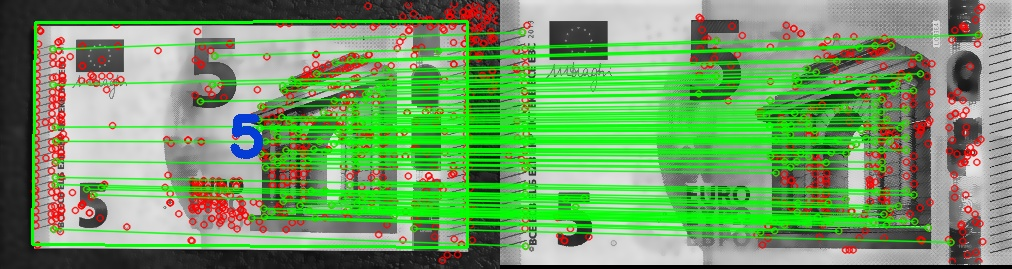
\includegraphics[width=0.36\textwidth]{notes-recognition/5__(5).jpg___SIFT-Detector_SIFT-Extractor_BF-Matcher_lowQualityImageDB_globalMatch__inliersMatches__0}\hfill
	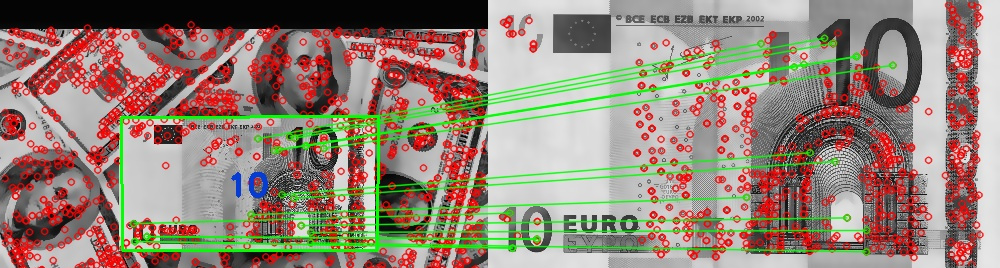
\includegraphics[width=0.36\textwidth]{notes-recognition/10__(9).jpeg___SIFT-Detector_SIFT-Extractor_BF-Matcher_lowQualityImageDB_globalMatch__inliersMatches__0}
	\caption{Detection of a banknote in an ideal perspective view with (bottom) and without (top) background clutter (using SIFT detector, SIFT descriptors and BFMatcher)}
	\label{fig:recognition-clutter}
\end{figure}

\begin{figure}[H]
	\centering
	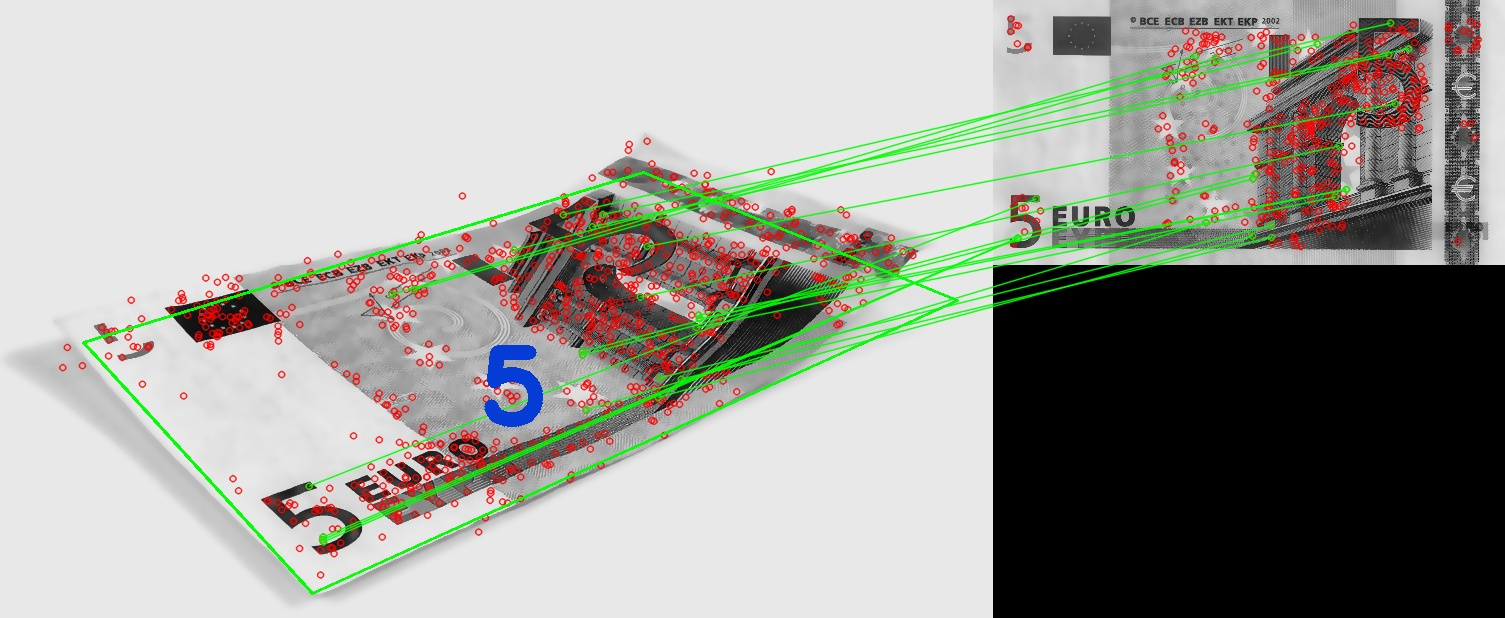
\includegraphics[width=0.36\textwidth]{notes-recognition/5__(6).jpg___SURF-Detector_SURF-Extractor_BF-Matcher_lowQualityImageDB_globalMatch__inliersMatches__0}\hfill
	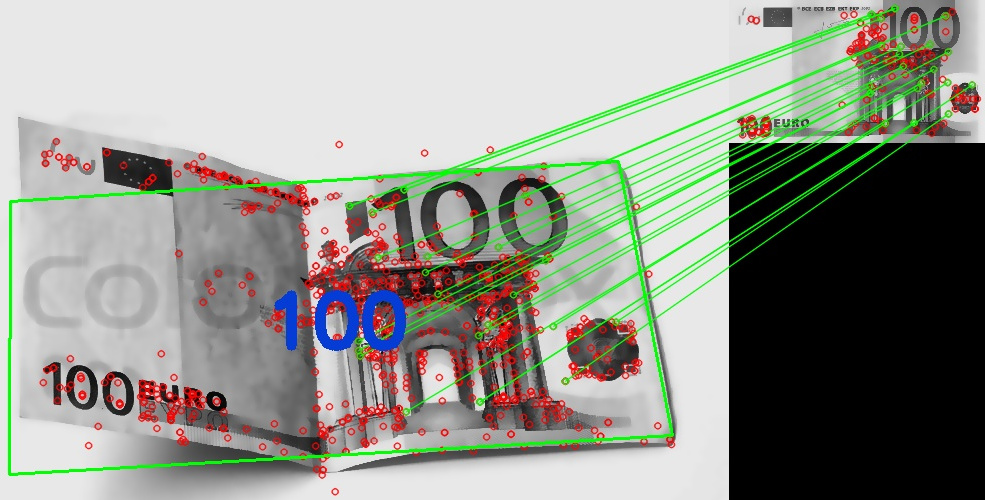
\includegraphics[width=0.36\textwidth]{notes-recognition/100__(4).jpg___SIFT-Detector_SIFT-Extractor_BF-Matcher_dynamicQualityImageDB_globalMatch__inliersMatches__0.jpg}
	\caption{Detection of banknotes with perspective distortion and folding (left image used SURF detector, SURF descriptors and BFMatcher while the right image used SIFT detector, SIFT descriptors and BFMatcher)}
	\label{fig:recognition-perspective-distortion}
\end{figure}


\begin{figure}[H]
	\centering
	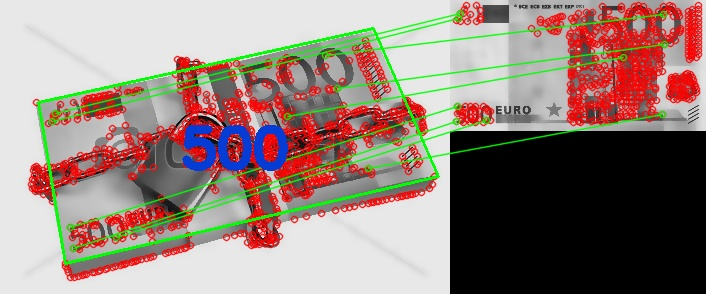
\includegraphics[width=0.405\textwidth]{notes-recognition/500.jpg___GFTT-Detector_SIFT-Extractor_BF-Matcher_dynamicQualityImageDB_globalMatch__inliersMatches__0}\hfill
	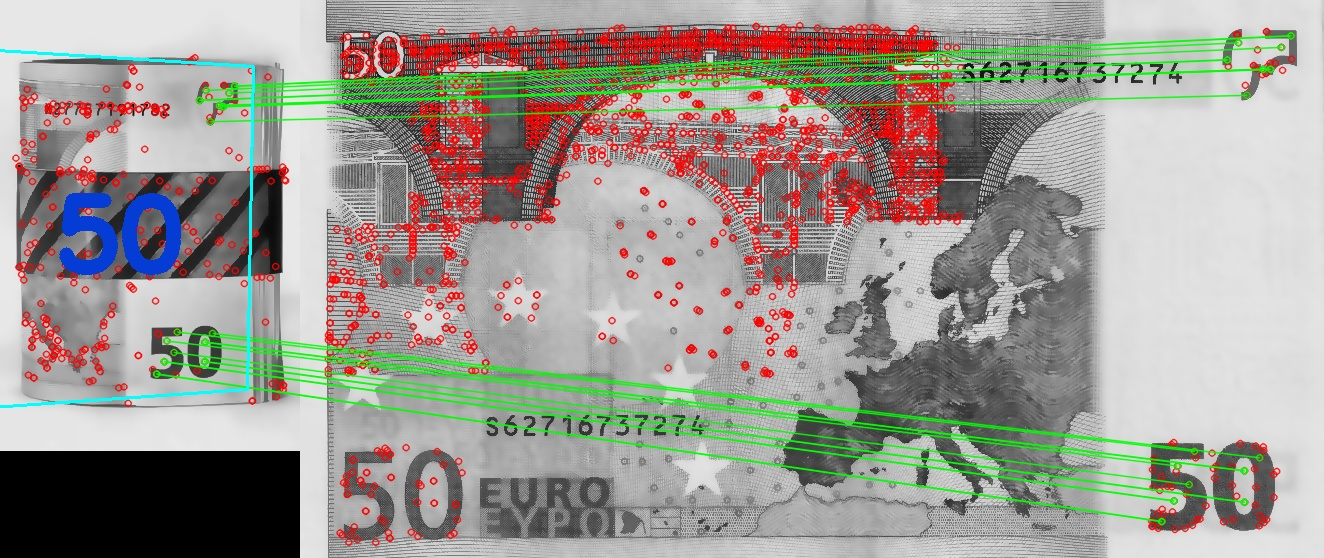
\includegraphics[width=0.405\textwidth]{notes-recognition/50__(13).jpg___SIFT-Detector_SIFT-Extractor_BF-Matcher_mediumQualityImageDB_globalMatch__inliersMatches__0}
	\caption{Detection of partially occluded banknotes (left image used GFTT detector, SIFT descriptors and BFMatcher while the right image used SIFT detector, SIFT descriptors and BFMatcher)}
	\label{fig:recognition-partially-occluded-banknotes}
\end{figure}

\begin{figure}[H]
	\centering
	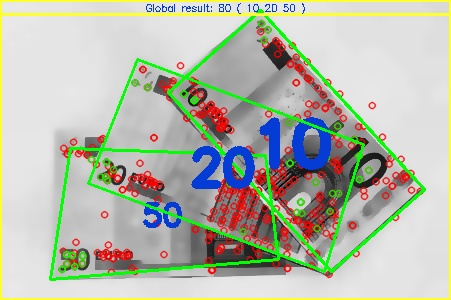
\includegraphics[width=0.405\textwidth]{notes-recognition/10-20-50.jpg___SIFT-Detector_SIFT-Extractor_BF-Matcher_dynamicQualityImageDB_globalMatch}
	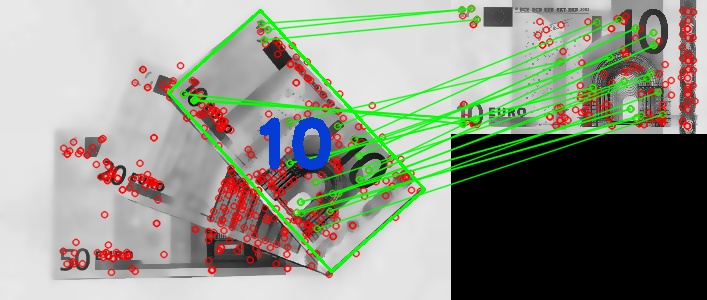
\includegraphics[width=0.405\textwidth]{notes-recognition/10-20-50.jpg___SIFT-Detector_SIFT-Extractor_BF-Matcher_dynamicQualityImageDB_globalMatch__inliersMatches__1}
	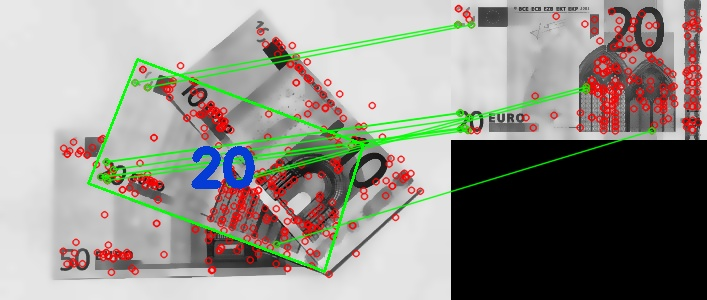
\includegraphics[width=0.405\textwidth]{notes-recognition/10-20-50.jpg___SIFT-Detector_SIFT-Extractor_BF-Matcher_dynamicQualityImageDB_globalMatch__inliersMatches__2}
	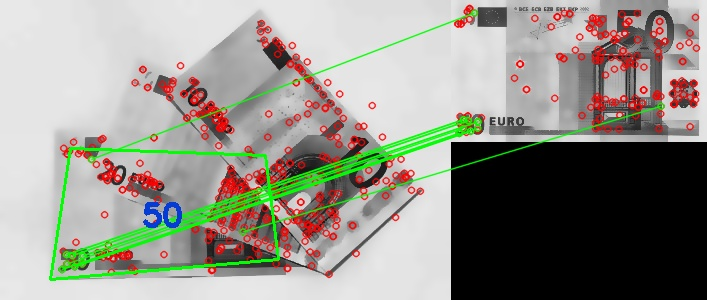
\includegraphics[width=0.405\textwidth]{notes-recognition/10-20-50.jpg___SIFT-Detector_SIFT-Extractor_BF-Matcher_dynamicQualityImageDB_globalMatch__inliersMatches__0}
	\caption{Detection of overlapping banknotes (using SIFT detector, SIFT descriptors and BFMatcher)}
	\label{fig:recognition-overlapping-banknotes}
\end{figure}

\section{Analysis of Results}\label{sec:results-analysis}

Analyzing \cref{fig:recognition-clutter,fig:recognition-perspective-distortion,fig:recognition-partially-occluded-banknotes,fig:recognition-overlapping-banknotes} it can be seen that the proposed recognition system managed to correctly detect the Euro banknotes with perspective distortion and folding (shown in \cref{fig:recognition-perspective-distortion}) and also with partial occlusion (presented in \cref{fig:recognition-partially-occluded-banknotes}). Moreover, it was able to detect several overlapping banknotes in the same image (seen in \cref{fig:recognition-overlapping-banknotes}). Optimal contour estimation was achieved with banknotes without folding and few perspective distortion (example in \cref{fig:recognition-clutter}).

Several configurations were tested by combining different feature detectors with feature descriptors, and also using different approaches to perform the descriptor matching and inliers filtering. Analyzing \cref{tab:recognition-configurations} it can be seen that the configuration using \gls{sift} as detector and descriptor in conjunction with a brute force matcher achieved best recognition results. The best performance of \gls{sift} is mainly related to the fact that it can select feature points that can be reliably detected even if the objects are in different perspective views. Moreover, it can compute descriptors that are robust to different lighting conditions. For real-time use, the \gls{surf} feature detector and descriptor algorithms are more suitable, since they achieve similar results with significant less computation time. This is achieved mainly due to the simplification of the computations by using integral images. The brute force matcher, although slower than \gls{flann}, achieved better results because unlike the heuristic approach, it matches all descriptors in order to find the best correspondences. However, if the system is to be used in real time, \gls{flann} can be employed with very similar results and lower computation time. In relation to the inliers filtering method, the best results were achieved when the best matched reference image was selected based on the global inliers ratio. However for test images in which most of the banknotes regions were occluded, the local inliers ratio performed better. This occurred because the local matching of patches avoids the removal of recognition results that have low inliers ratio.

\section{Conclusions}\label{sec:conclusions}

The proposed recognition system successfully recognized the 95 banknotes in the 80 test images, even when they had significant perspective distortion or were partially occluded. It was also robust enough to handle folded and wrinkled banknotes with different kinds of illumination. This was achieved by carefully identifying the regions of the banknotes that had unique features in order to avoid the usage of structures that were similar between banknotes. This technique in conjunction with the usage of reference images with several levels of detail were crucial to improve the correct matching of keypoints descriptors and ensure the correct recognition of the banknotes. The system was configured to recognize Euro banknotes, but can easily be reconfigured to detect other currencies. The achieved results make it a viable option to be used by visually impaired people or to improve automatic banknote counting machines and even increase the security of \glspl{atm} by detecting counterfeit banknotes.

Future work would include the test of the system using the banknotes under ultra-violet and infra-red light in order to detect with higher confidence counterfeit banknotes and also integrate the system with a speech synthesizer in order to be usable by blind people.

\section*{Acknowledgments}\label{sec:acknowledgments}

Acknowledgments text.




%---------------------------------------------------------------------------------------------------
% Bibliography
%---------------------------------------------------------------------------------------------------

\bibliographystyle{IEEEtran}
\bibliography{references}


\end{document}
